%% FullCourse_10Lecs -- Lecture 8, Topic 8.2: RAG Principled + Chunking + Embeddings
%% Source: ./archive_pre_split/Lec08_RAG.tex (sections 4-6)
%% Pass B (2026-05-17): diffed against
%%         ../../MiniCourse_8hr/Slides/Module4_Agentic_AI/M4_T1_RAG_Foundations.tex
%% No new frames ported -- FullCourse T2 is already a strict superset of MiniCourse
%% M4_T1 (which compresses chunking + embeddings into single overview frames).
%% All existing FullCourse frames retained.

%% Shared preamble for the FullCourse_10Lecs topic decks.
%%
%% Each topic .tex \input's this file, then defines its own \title, \date
%% override (if any), \graphicspath, and \begin{document}.
%%
%% Reconstructed verbatim from the inlined copy preserved in
%% Lec10_Case_Studies/Lec10_T8_Case6_DeepRamsey.tex (lines 23-190), which is
%% explicitly annotated there as "from ../shared_preamble.tex, copied verbatim".
%% Base preamble matches MiniCourse_8hr/Slides/shared_preamble.tex; this version
%% additionally provides \sectiondivider, the conceptbox/cautionbox/examplebox/
%% takeawaybox tcolorboxes, and \compacttables used across the split decks.

\documentclass[10pt,english,aspectratio=169]{beamer}

\usepackage{ae,aecompl}
\usepackage[T1]{fontenc}
\usepackage{textcomp}
\usepackage[utf8]{inputenc}
\usepackage{babel}
\usepackage{datetime2}

\setcounter{secnumdepth}{3}
\setcounter{tocdepth}{3}

\usepackage{amsmath, amssymb, amsthm, graphicx}
\usepackage{booktabs, multirow}
\usepackage{tikz}
\usepackage{pgfplots}
\pgfplotsset{compat=1.16}
\usepackage[most]{tcolorbox}
\tcbuselibrary{skins, breakable, theorems}
\usepackage{listings}
\usepackage{xcolor}

\lstset{
  basicstyle=\ttfamily\small,
  keywordstyle=\color{blue!80!black}\bfseries,
  commentstyle=\color{green!50!black}\itshape,
  stringstyle=\color{orange!80!black},
  backgroundcolor=\color{gray!8},
  frame=single,
  rulecolor=\color{gray!40},
  breaklines=true,
  showstringspaces=false,
  numbers=none,
}

\lstdefinestyle{pythonstyle}{
    language=Python,
    basicstyle=\ttfamily\footnotesize,
    keywordstyle=\color{blue!80!black}\bfseries,
    commentstyle=\color{green!50!black}\itshape,
    stringstyle=\color{orange!80!black},
    frame=single,
    breaklines=true,
    showstringspaces=false,
    numbers=left,
    numbersep=5pt,
    numberstyle=\tiny\color{gray},
    backgroundcolor=\color{gray!8},
    rulecolor=\color{gray!40}
}

\ifx\hypersetup\undefined
  \AtBeginDocument{%
    \hypersetup{bookmarks=false,breaklinks=true,pdfborder={0 0 0},colorlinks=true,
      linkcolor=DarkText,urlcolor=RedTitle}%
  }
\else
  \hypersetup{bookmarks=false,breaklinks=true,pdfborder={0 0 0},colorlinks=true,
    linkcolor=DarkText,urlcolor=RedTitle}%
\fi

\makeatletter
\newcommand\makebeamertitle{%
  \begin{frame}[plain]
    \vspace*{1.0cm}
    \centering
    {\usebeamerfont{title}\usebeamercolor[fg]{title}\inserttitle\par}
    \vspace{1.0cm}
    {\usebeamerfont{author}\usebeamercolor[fg]{author}\insertauthor\par}
    \vspace{0.2cm}
    {\usebeamerfont{date}\usebeamercolor[fg]{date}\insertdate\par}
  \end{frame}}%
\AtBeginDocument{%
  \let\origtableofcontents=\tableofcontents
  \def\tableofcontents{\@ifnextchar[{\origtableofcontents}{\gobbletableofcontents}}
  \def\gobbletableofcontents#1{\origtableofcontents}%
}

\usetheme{metropolis}
\usefonttheme{professionalfonts}

\definecolor{LightGray}{RGB}{230,230,230}
\definecolor{RedTitle}{RGB}{0,0,200}
\definecolor{VeryLightGray}{RGB}{245,245,245}
\definecolor{DarkText}{RGB}{0,0,0}

\setbeamercolor{background canvas}{bg=white}
\setbeamercolor{title}{fg=RedTitle}
\setbeamercolor{author}{fg=DarkText}
\setbeamercolor{date}{fg=DarkText}
\setbeamercolor{frametitle}{bg=VeryLightGray,fg=DarkText}
\setbeamercolor{normal text}{fg=DarkText}
\setbeamerfont{title}{size=\large}

\setbeamersize{text margin left=5mm, text margin right=5mm}
\addtobeamertemplate{frametitle}{}{\vspace{-0.5em}}
\newcommand{\reducevspace}{\vspace{-0.5cm}}

% Shared section divider and box styles for split topic decks.
\newcommand{\sectiondivider}[2]{%
\begin{frame}[plain,noframenumbering]
\begin{center}
\vfill
{\Large\textbf{#1}\par}
\vspace{0.35cm}
{\normalsize #2\par}
\vfill
\end{center}
\end{frame}
}

\newtcolorbox{conceptbox}[1][]{
  colback=blue!3,
  colframe=RedTitle!55,
  boxrule=0.35mm,
  arc=1mm,
  left=2mm,
  right=2mm,
  top=1mm,
  bottom=1mm,
  #1
}
\newtcolorbox{cautionbox}[1][]{
  colback=red!3,
  colframe=red!50!black,
  boxrule=0.35mm,
  arc=1mm,
  left=2mm,
  right=2mm,
  top=1mm,
  bottom=1mm,
  #1
}
\newtcolorbox{examplebox}[1][]{
  colback=green!3,
  colframe=green!45!black,
  boxrule=0.35mm,
  arc=1mm,
  left=2mm,
  right=2mm,
  top=1mm,
  bottom=1mm,
  #1
}
\newtcolorbox{takeawaybox}[1][]{
  colback=VeryLightGray,
  colframe=RedTitle!55,
  boxrule=0.35mm,
  arc=1mm,
  left=2mm,
  right=2mm,
  top=1mm,
  bottom=1mm,
  #1
}
\newcommand{\compacttables}{\renewcommand{\arraystretch}{1.15}}

\setbeamertemplate{navigation symbols}{}
\setbeamertemplate{footline}{%
  \hfill%
  \usebeamercolor[fg]{page number in head/foot}%
  \usebeamerfont{page number in head/foot}%
  \insertframenumber\,/\,\inserttotalframenumber\kern1em\vskip2pt%
}

\makeatother

\author{Zhigang Feng}
% "date with time": compile timestamp so each build is identifiable.
\date{\today\ \DTMcurrenttime}


\usetikzlibrary{arrows.meta, positioning, shapes.geometric, fit, calc, backgrounds}

\graphicspath{{./pic/}{./figures/}{../../MiniCourse_8hr/Slides/Module4_Agentic_AI/pic/}{../}}

\title[AI for Econ Research]{AI for Economic Research: Dynamic Models, Language, and Agents\\
Lecture 8.2: RAG --- Chunking and Embeddings}

\begin{document}

\makebeamertitle

%=============================================================================
\begin{frame}{Topic 8.2 Agenda}
\begin{enumerate}
  \item \textbf{RAG --- The Principled Solution}
  \medskip
  \item \textbf{Chunking}
  \medskip
  \item \textbf{Embeddings} --- dense vector representations
\end{enumerate}

\medskip
\textit{Arc: T1 Prompting wall $\to$ \textbf{T2 Chunking \& embeddings} $\to$ T3 Vector \& graph retrieval $\to$ T4a Augmented generation $\to$ T4b Demo, failures, agentic bridge}
\end{frame}

%=============================================================================
\section{RAG --- The Principled Solution}

\begin{frame}{The Institutional-Memory Picture: Offline Index vs Online Query}
\begin{center}
\begin{tikzpicture}[
  font=\footnotesize,
  node distance=0.45cm and 0.6cm,
  off/.style={draw, rounded corners=2pt, minimum width=1.85cm, minimum height=0.65cm, align=center, fill=blue!7},
  on/.style={draw, rounded corners=2pt, minimum width=1.85cm, minimum height=0.65cm, align=center, fill=orange!12},
  store/.style={draw, cylinder, shape border rotate=90, aspect=0.25, minimum width=2.0cm, minimum height=1.2cm, align=center, fill=blue!10},
  arr/.style={-{Latex[length=2.0mm]}, thick}
]
  % Top row: Offline Phase
  \node[font=\small\bfseries, anchor=west] at (-0.3, 2.7) {Offline Phase (do once; index = institutional memory)};
  \node[off] (docs)   at (0.5, 1.7) {Collect\\(PDF, HTML)};
  \node[off] (chunk)  at (3.2, 1.7) {Chunk\\(+ metadata)};
  \node[off] (emb1)   at (5.9, 1.7) {Embed\\(transformer)};
  \node[store] (db)   at (8.8, 0.45) {Vector\\Store};
  \draw[arr] (docs) -- (chunk);
  \draw[arr] (chunk) -- (emb1);
  \draw[arr] (emb1.east) -- ++(0.6,0) |- (db.north);

  % Bottom row: Online Phase
  \node[font=\small\bfseries, anchor=west] at (-0.3, -0.55) {Online Phase (do every query; cheap, cached, audit-friendly)};
  \node[on] (q)       at (0.5, -1.55) {User\\Query};
  \node[on] (emb2)    at (3.2, -1.55) {Embed\\(same model)};
  \node[on] (retr)    at (5.9, -1.55) {Top-$K$\\Retrieve};
  \node[on] (gen)     at (8.8, -1.55) {Augmented\\Generate};
  \node[on] (ans)     at (11.6, -1.55) {Cited\\Answer};
  \draw[arr] (q) -- (emb2);
  \draw[arr] (emb2) -- (retr);
  \draw[arr] (db.south) |- (retr.west);
  \draw[arr] (retr) -- (gen);
  \draw[arr] (gen) -- (ans);

  % Visual separator
  \draw[gray, dashed] (-0.5, 0.5) -- (12.5, 0.5);
\end{tikzpicture}
\end{center}

\smallskip
\begin{itemize}\small
\item \textbf{Offline (blue)} is the costly, one-time work --- build the index over the FOMC / NBER / 10-K archive.
\item \textbf{Online (orange)} is the cheap, repeated work --- one query embeds once, retrieves the top-$K$, ships only that to the LLM.
\item \textbf{The separation is the point}: the same index supports thousands of queries over months without re-paying the ingestion bill.
\end{itemize}
\end{frame}

\begin{frame}{The Key Insight}
\begin{itemize}
\item Don't paste the whole corpus into every prompt.

\medskip
\item Instead:
\begin{enumerate}
    \item \textbf{Pre-process documents once.} Split them into chunks, convert each chunk to a numerical fingerprint (an \emph{embedding}), store everything in a database.
    \item \textbf{At query time, fetch only what's relevant.} Convert the user's question to an embedding, look up the closest chunks in the database, paste \emph{those few chunks} into the prompt.
    \item \textbf{Let the LLM answer from the retrieved evidence}, citing which chunks it used.
\end{enumerate}

\medskip
\item This is a \textbf{two-phase architecture:}
\begin{itemize}
    \item \emph{Offline:} index everything once.
    \item \emph{Online:} retrieve a few relevant pieces per query, generate the answer.
\end{itemize}

\medskip
\item Cost is now proportional to \emph{what you actually need}, not to the size of the corpus. Storage is amortized. Indexes are updatable. The model only ever sees relevant text, so quality and faithfulness improve.
\end{itemize}
\end{frame}

\begin{frame}{Definition}
\begin{itemize}
\item \textbf{Retrieval Augmented Generation (RAG):}\\
A system that, before answering a query, \emph{retrieves} relevant documents from an external knowledge store and supplies them to a language model as additional context for \emph{generation}.

\medskip
\item \textbf{Origin:} Lewis, Perez, Piktus, et al.\ (2020), \emph{``Retrieval-Augmented Generation for Knowledge-Intensive NLP Tasks,''} NeurIPS.

\medskip
\item Originally framed as a research architecture for open-domain QA. Now the \emph{de facto} production pattern for any LLM application that touches a custom knowledge base: customer-support bots, legal research, medical Q\&A, code search, and academic research.

\medskip
\item \textbf{Key idea (worth repeating):} The LLM is the \emph{reasoner}. The vector store is the \emph{memory}. The retriever is the \emph{librarian}. RAG is how we connect them.
\end{itemize}
\end{frame}

\begin{frame}{End-to-End Architecture}
\begin{center}
\begin{tikzpicture}[
  font=\small,
  node distance=0.7cm and 0.9cm,
  box/.style={draw, rounded corners=2pt, minimum width=2.0cm, minimum height=0.8cm, align=center, fill=VeryLightGray},
  store/.style={draw, cylinder, shape border rotate=90, aspect=0.25, minimum width=2.0cm, minimum height=1.1cm, align=center, fill=blue!8},
  llm/.style={draw, rounded corners=2pt, minimum width=2.2cm, minimum height=1.0cm, align=center, fill=orange!10},
  arr/.style={-{Latex[length=2.2mm]}, thick}
]
  \node[box] (q) {User\\Query};
  \node[box, right=of q] (emb) {Embedder};
  \node[store, right=of emb] (db) {Vector\\Store};
  \node[box, right=of db] (top) {Top-$K$\\Chunks};
  \node[llm, below=of top] (llm) {LLM\\(generator)};
  \node[box, left=of llm] (ctx) {Augmented\\Prompt};
  \node[box, left=of ctx] (ans) {Grounded\\Answer};

  \draw[arr] (q) -- (emb);
  \draw[arr] (emb) -- (db);
  \draw[arr] (db) -- (top);
  \draw[arr] (top) -- (llm);
  \draw[arr] (llm) -- (ctx);
  \draw[arr] (ctx) -- (ans);
\end{tikzpicture}
\end{center}

\medskip
\textbf{Five components:}
\begin{enumerate}
\item \textbf{Embedder} --- maps text to vectors (Section V).
\item \textbf{Vector store} --- holds embeddings of every chunk (Section VI).
\item \textbf{Retriever} --- pulls the top-$K$ closest chunks to the query.
\item \textbf{Augmented prompt} --- retrieved chunks + user question + instructions (Section VII).
\item \textbf{Generator} --- the LLM that writes the final answer.
\end{enumerate}
\end{frame}

\begin{frame}{Two Phases --- Offline Indexing}
\begin{center}
\begin{tikzpicture}[
  font=\small,
  node distance=0.6cm and 0.9cm,
  box/.style={draw, rounded corners=2pt, minimum width=2.0cm, minimum height=0.8cm, align=center, fill=VeryLightGray},
  store/.style={draw, cylinder, shape border rotate=90, aspect=0.25, minimum width=2.0cm, minimum height=1.1cm, align=center, fill=blue!8},
  arr/.style={-{Latex[length=2.2mm]}, thick}
]
  \node[box] (docs) {Documents\\(PDFs, HTML)};
  \node[box, right=of docs] (chunk) {Chunker};
  \node[box, right=of chunk] (emb) {Embedder};
  \node[store, right=of emb] (db) {Vector\\Store};

  \draw[arr] (docs) -- (chunk);
  \draw[arr] (chunk) -- (emb);
  \draw[arr] (emb) -- (db);
\end{tikzpicture}
\end{center}

\medskip
\begin{itemize}
\item Done \textbf{once} --- or incrementally as new documents arrive.
\item Cost is paid up front; queries are then cheap.
\item \textbf{Library catalog analogy:} Building the card catalog is slow work. Once it exists, looking things up is fast.
\item \textbf{For an economist:} Index the entire FOMC archive (1993--present) one weekend; then query it for years.
\end{itemize}
\end{frame}

\begin{frame}{Two Phases --- Online Query}
\begin{center}
\begin{tikzpicture}[
  font=\small,
  node distance=0.55cm and 0.7cm,
  box/.style={draw, rounded corners=2pt, minimum width=1.7cm, minimum height=0.75cm, align=center, fill=VeryLightGray},
  store/.style={draw, cylinder, shape border rotate=90, aspect=0.25, minimum width=1.7cm, minimum height=1.0cm, align=center, fill=blue!8},
  llm/.style={draw, rounded corners=2pt, minimum width=1.7cm, minimum height=0.9cm, align=center, fill=orange!10},
  arr/.style={-{Latex[length=2mm]}, thick}
]
  \node[box] (q) {Query};
  \node[box, right=of q] (emb) {Embedder};
  \node[store, right=of emb] (db) {Vector\\Store};
  \node[box, right=of db] (top) {Top-$K$};
  \node[box, right=of top] (prompt) {Augmented\\Prompt};
  \node[llm, right=of prompt] (llm) {LLM};
  \node[box, right=of llm] (ans) {Answer};

  \draw[arr] (q) -- (emb);
  \draw[arr] (emb) -- (db);
  \draw[arr] (db) -- (top);
  \draw[arr] (top) -- (prompt);
  \draw[arr] (prompt) -- (llm);
  \draw[arr] (llm) -- (ans);
\end{tikzpicture}
\end{center}

\medskip
\begin{itemize}
\item Done \textbf{every time the user asks a question}.
\item Each query embeds once, retrieves a handful of chunks, and pays for only those tokens at the LLM stage.
\item \textbf{Ask-the-librarian analogy:} You walk up with a question, the librarian hands you 5 relevant pages, you read them and answer.
\item \textbf{Use the same embedder for indexing and querying} --- otherwise the geometry doesn't line up.
\end{itemize}
\end{frame}

%=============================================================================
\section{Chunking}

\begin{frame}{Why Chunk At All?}
\begin{itemize}
\item Documents are too big to embed as a single vector. We must split them into smaller pieces --- \emph{chunks} --- before indexing.

\medskip
\item \textbf{Three reasons to chunk:}
\begin{enumerate}
    \item \textbf{Embedder input limits.} Most embedding models accept 512--8192 tokens per input. A 60-page FOMC transcript blows past every limit.
    \item \textbf{Granularity of relevance.} If you index a whole 30-page document as one vector, the embedding averages over many topics. A query about ``inflation expectations'' may match a document that contains \emph{one paragraph} on the topic --- but the average vector won't reflect it.
    \item \textbf{Generator context budget.} You only inject a few chunks into the LLM prompt. Smaller chunks $\Rightarrow$ more chunks fit $\Rightarrow$ richer evidence base.
\end{enumerate}

\medskip
\item \textbf{Trade-off:} Chunks too large $\Rightarrow$ noisy embeddings. Chunks too small $\Rightarrow$ context lost. \emph{Choosing chunk size is the most consequential decision in a RAG pipeline.}
\end{itemize}
\end{frame}

\begin{frame}{Chunking Strategies --- The Trade-Off, Visually}
\begin{center}
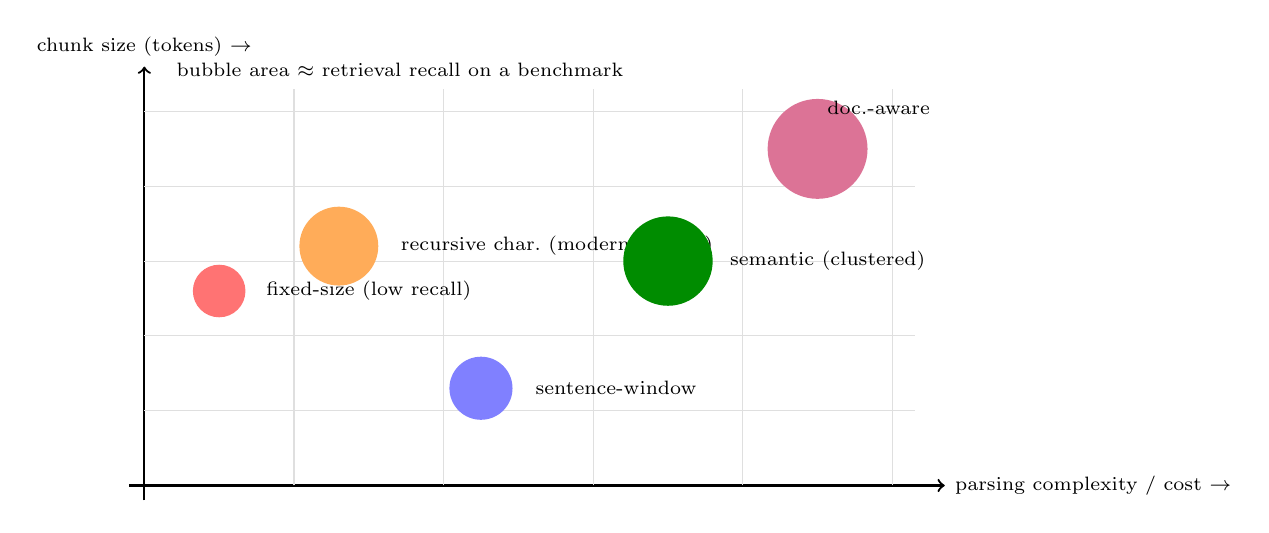
\begin{tikzpicture}[font=\footnotesize, scale=0.95]
  % axes
  \draw[->, thick] (-0.2,0) -- (10.7,0) node[right, font=\scriptsize] {parsing complexity / cost $\to$};
  \draw[->, thick] (0,-0.2) -- (0,5.6) node[above, font=\scriptsize] {chunk size (tokens) $\to$};
  % light gridlines
  \foreach \x in {2,4,6,8,10} \draw[gray!25] (\x,0) -- (\x,5.3);
  \foreach \y in {1,2,3,4,5} \draw[gray!25] (0,\y) -- (10.3,\y);

  % Strategy bubbles: (x = complexity, y = chunk-size, r = retrieval-recall on benchmark)
  % Fixed-size: low complexity, mid size, low recall
  \fill[red!55] (1.0,2.6) circle (10pt);
  \node[font=\scriptsize, anchor=west] at (1.5,2.6) {fixed-size (low recall)};

  % Recursive character: low-mid complexity, mid size, mid-high recall
  \fill[orange!65] (2.6,3.2) circle (15pt);
  \node[font=\scriptsize, anchor=west] at (3.3,3.2) {recursive char.\ (modern default)};

  % Sentence-window: mid complexity, small size, mid recall
  \fill[blue!50] (4.5,1.3) circle (12pt);
  \node[font=\scriptsize, anchor=west] at (5.1,1.3) {sentence-window};

  % Semantic: high complexity, variable mid size, high recall but expensive
  \fill[green!55!black] (7.0,3.0) circle (17pt);
  \node[font=\scriptsize, anchor=west] at (7.7,3.0) {semantic (clustered)};

  % Document-aware: highest complexity for structured corpora, large size, highest recall
  \fill[purple!55] (9.0,4.5) circle (19pt);
  \node[font=\scriptsize, anchor=west] at (9.0,5.05) {doc.-aware};

  % Legend
  \node[font=\scriptsize, anchor=west] at (0.3,5.55) {bubble area $\approx$ retrieval recall on a benchmark};
\end{tikzpicture}
\end{center}

\smallskip
\textbf{Practical recommendation:} start with \emph{recursive character} (LangChain default --- big orange bubble, low setup cost). Move \emph{up the y-axis to document-aware} when the corpus has rich structure (FOMC, 10-K, Congress). Reach for \emph{semantic} only after you have measured retrieval quality and can justify the embedding-pass cost.
\end{frame}

\begin{frame}{Fixed-Size vs.\ Recursive --- An Example}
\begin{itemize}
\item \textbf{Source paragraph} (FOMC minutes, simplified):
\begin{quote}
\small\itshape
``Participants observed that inflation remained elevated. Several noted that core services prices, especially shelter, continued to rise. A few participants expressed concern about persistence in wage growth. Most agreed that policy should remain restrictive.''
\end{quote}

\medskip
\item \textbf{Fixed 60-character chunks:}
\begin{quote}
\small\ttfamily
{[}``Participants observed that inflation remained elevat''] \\
{[}``ed. Several noted that core services prices, especi''] \\
{[}``ally shelter, continued to rise. A few participants''] \dots
\end{quote}
$\Rightarrow$ \textbf{Cuts mid-word.} Embeddings of these fragments are nearly useless.

\medskip
\item \textbf{Recursive chunking} (split on paragraph $\to$ sentence $\to$ word, target $\sim$120 chars):
\begin{quote}
\small\ttfamily
[``Participants observed that inflation remained elevated.''] \\
{[}``Several noted that core services prices, especially shelter, continued to rise.''] \\
{[}``A few participants expressed concern about persistence in wage growth.'']
\end{quote}
$\Rightarrow$ Each chunk is a self-contained sentence. Embeddings carry meaning.
\end{itemize}
\end{frame}

\begin{frame}{Semantic Chunking}
\begin{itemize}
\item \textbf{Idea:} Don't fix chunk size in advance. Instead, embed each sentence, measure similarity between adjacent sentences, and split where the similarity \emph{drops} --- i.e., where the topic changes.

\medskip
\item \textbf{Algorithm sketch:}
\begin{enumerate}
    \item Split the document into sentences.
    \item Embed each sentence with a fast embedder.
    \item Compute cosine similarity between consecutive sentence embeddings.
    \item Mark a chunk boundary wherever similarity falls below a threshold (or a percentile cutoff).
\end{enumerate}

\medskip
\item \textbf{Pros:} Each chunk is topically coherent --- you don't slice mid-thought.

\medskip
\item \textbf{Cons:} Costs an embedding pass over every sentence \emph{at indexing time}. For very large corpora this is non-trivial.

\medskip
\item \textbf{When to use:} When recursive chunking gives noisy retrieval and you have evidence that within-document topic shifts matter (long technical reports, multi-section speeches).
\end{itemize}
\end{frame}

\begin{frame}[fragile]{Practical Defaults + Code}
\begin{itemize}
\item \textbf{Sensible defaults} for institutional text:
\begin{itemize}
    \item Chunk size: 500--1000 tokens ($\sim$2--4 paragraphs)
    \item Chunk overlap: 10--20\% (so a sentence on a chunk boundary appears in both neighbors)
    \item \textbf{Always preserve metadata}: doc ID, page number, section heading, date, author
\end{itemize}

\medskip
\item \textbf{LangChain recursive chunker} (the de facto standard):
\begin{lstlisting}[language=Python]
from langchain.text_splitter import RecursiveCharacterTextSplitter

splitter = RecursiveCharacterTextSplitter(
    chunk_size=800,            # ~600 tokens
    chunk_overlap=100,         # ~80 tokens of overlap
    separators=["\n\n", "\n", ". ", " ", ""],
)

chunks = splitter.create_documents(
    texts=[fomc_minutes_text],
    metadatas=[{"meeting": "2024-06", "doc_type": "minutes"}],
)
\end{lstlisting}
\end{itemize}
\end{frame}

\begin{frame}{The Economist's Chunking Gotcha}
\begin{itemize}
\item Real institutional documents have \textbf{structure} that naive chunkers destroy.

\medskip
\item \textbf{FOMC minutes:} organized as \emph{speaker turns}. ``Participants generally agreed\dots'', ``A few members noted\dots''. Cutting across speaker boundaries fuses unrelated viewpoints.

\medskip
\item \textbf{Congressional Record:} hierarchical metadata --- Congress / session / chamber / date / speaker / bill. Lose the hierarchy and you can't filter or cite properly.

\medskip
\item \textbf{SEC 10-K filings:} standardized item numbers (Item 1, Item 1A Risk Factors, Item 7 MD\&A). A query about ``risk factors'' should retrieve only \emph{Item 1A} content --- which only works if you parse the structure first.

\medskip
\item \textbf{Practical fix:} Write a corpus-specific parser that emits chunks with rich metadata. Extra effort up front; massive payoff in retrieval quality and ability to filter.

\medskip
\item \textbf{Lesson:} Don't reach for the generic chunker. Let your corpus tell you what a chunk should be.
\end{itemize}
\end{frame}

%=============================================================================
\section{Embeddings}

\begin{frame}{From Text to Vectors --- What and Why}
\begin{itemize}
\item An \textbf{embedding} is a function $E: \text{text} \to \mathbb{R}^d$ that maps a piece of text to a fixed-length vector of real numbers.

\medskip
\item Typical dimensionalities: $d \in \{384, 768, 1024, 1536, 3072\}$.

\medskip
\item \textbf{The crucial property:}
\[
\text{semantically similar texts } \;\Longrightarrow\; \text{nearby vectors in } \mathbb{R}^d
\]

\medskip
\item \textbf{Why this is useful:} Once your corpus lives in a vector space, ``find documents about inflation expectations'' becomes a \emph{geometric} operation: compute the embedding of the query, find its nearest neighbors among the document embeddings.

\medskip
\item \textbf{Recap from Lec.\ 7:} Embeddings appear \emph{inside} the transformer (token embeddings). Here we use the \emph{sentence-} or \emph{document-level} embedding produced by a separate retrieval-tuned model.
\end{itemize}
\end{frame}

\begin{frame}{Geometric Intuition}
\begin{center}
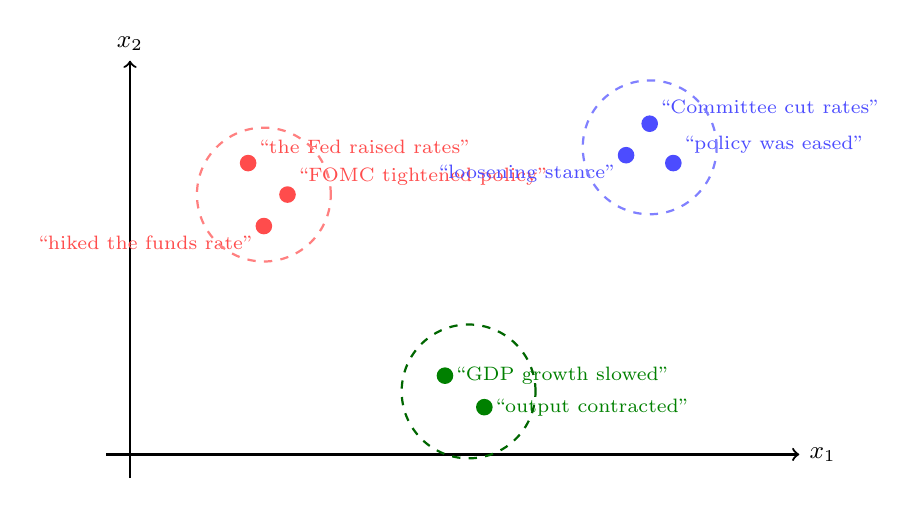
\begin{tikzpicture}[font=\small, scale=1.0]
  \draw[->, thick] (-0.3,0) -- (8.5,0) node[right] {$x_1$};
  \draw[->, thick] (0,-0.3) -- (0,5.0) node[above] {$x_2$};

  % Cluster A: hawkish / tightening
  \fill[red!70] (1.5,3.7) circle (3pt) node[above right, font=\scriptsize] {``the Fed raised rates''};
  \fill[red!70] (2.0,3.3) circle (3pt) node[above right, font=\scriptsize] {``FOMC tightened policy''};
  \fill[red!70] (1.7,2.9) circle (3pt) node[below left, font=\scriptsize] {``hiked the funds rate''};
  \draw[red!50, thick, dashed] (1.7,3.3) circle (0.85);

  % Cluster B: dovish / easing
  \fill[blue!70] (6.6,4.2) circle (3pt) node[above right, font=\scriptsize] {``Committee cut rates''};
  \fill[blue!70] (6.9,3.7) circle (3pt) node[above right, font=\scriptsize] {``policy was eased''};
  \fill[blue!70] (6.3,3.8) circle (3pt) node[below left, font=\scriptsize] {``loosening stance''};
  \draw[blue!50, thick, dashed] (6.6,3.9) circle (0.85);

  % Cluster C: unrelated
  \fill[green!50!black] (4.0,1.0) circle (3pt) node[right, font=\scriptsize] {``GDP growth slowed''};
  \fill[green!50!black] (4.5,0.6) circle (3pt) node[right, font=\scriptsize] {``output contracted''};
  \draw[green!40!black, thick, dashed] (4.3,0.8) circle (0.85);
\end{tikzpicture}
\end{center}

\textbf{Reading the picture:}
\begin{itemize}
\item Hawkish-tightening sentences cluster on the left.
\item Dovish-easing sentences cluster on the right.
\item Unrelated growth-related sentences sit elsewhere.
\item Distance in vector space $\approx$ semantic distance in meaning.
\end{itemize}

\textbf{This is the picture every RAG pipeline relies on.}
\end{frame}

\begin{frame}{Why This Works --- Pooling + Contrastive Loss (Callback to Lec.\ 7 T2b)}
\begin{itemize}
\item \textbf{The transformer outputs one vector per token.} A \emph{retrieval embedder} pools those token vectors into a single \emph{document vector} (mean-pool, \texttt{[CLS]}, or a learned head). See Lec.\ 7 T2b ``Token Embeddings vs.\ Document Embeddings'' for the geometric derivation.

\medskip
\item \textbf{The pooled embedder is trained with a contrastive loss} on \emph{(query, positive, negative)} triples: pull semantically related text together, push unrelated text apart. The geometry is \emph{learned for similarity}, not inherited from the next-token objective.

\medskip
\item \textbf{Modern retrieval embedders} (\texttt{bge-large-en}, \texttt{voyage-3}, OpenAI \texttt{text-embedding-3}, Sentence-BERT lineage from Reimers \& Gurevych, 2019) all share this pattern. Differences are scale of training data and pooling head, not the core idea.

\medskip
\item \textbf{Take-away:} an embedder is a transformer encoder \emph{plus} a pooling head \emph{plus} a contrastive objective. Lec.\ 7 covered the encoder; Lec.\ 8 wires in the rest.
\end{itemize}
\end{frame}

\begin{frame}{Modern Embedding Models --- The Four You'll Actually Pick}
\begin{center}
\renewcommand{\arraystretch}{1.3}
\small
\begin{tabular}{|l|c|c|l|l|}
\hline
\textbf{Model} & \textbf{Dim} & \textbf{Cost} & \textbf{Hosting} & \textbf{Why pick it} \\
\hline
OpenAI \texttt{text-embedding-3-small} & 1536 & \$0.02/M & API & cheap default, no infra \\
\hline
OpenAI \texttt{text-embedding-3-large} & 3072 & \$0.13/M & API & top accuracy, paid \\
\hline
\texttt{voyage-3} & 1024 & \$0.06/M & API & top retrieval benchmarks \\
\hline
\texttt{bge-large-en-v1.5} & 1024 & free & local & best open-source local default \\
\hline
\end{tabular}
\end{center}

\smallskip
{\footnotesize\centering\textit{Model facts (dimensions and prices) current as of June 2026.}\par}

\bigskip
\textbf{For an academic researcher:}
\begin{itemize}
\item \textbf{Local + free:} \texttt{bge-large-en-v1.5}. Runs on a laptop GPU; competitive with paid APIs.
\item \textbf{Cloud + simple:} OpenAI \texttt{text-embedding-3-small}. Cheap, no infra.
\item \textbf{Top accuracy + budget:} \texttt{voyage-3} or OpenAI \texttt{3-large}.
\end{itemize}

\medskip
\footnotesize\textit{Full 7-row reference table (incl.\ Cohere, MiniLM, E5-Mistral) is in the deck appendix.}
\end{frame}

\begin{frame}{Economists' Embedding Example}
\begin{itemize}
\item \textbf{The setup.} Take every Federal Reserve Chair speech from 2010 to 2025 (Bernanke, Yellen, Powell). Embed each speech with \texttt{bge-large-en-v1.5}. Project to 2D with UMAP. Plot.

\medskip
\item \textbf{What you see:}
\begin{itemize}
    \item Crisis-era speeches (Bernanke 2010--2014) cluster together --- focused on QE, financial stability.
    \item Normalization-era speeches (Yellen 2015--2017) form a distinct cluster --- gradual exit, forward guidance.
    \item Pandemic and post-pandemic Powell (2020--2025) splits into two: 2020--2021 dovish ``patient'' speeches vs.\ 2022--2024 hawkish ``restrictive'' speeches.
\end{itemize}

\medskip
\item \textbf{Why this matters for research.} The clustering is generated \emph{purely from the text}, with no labels. The economist now has a reproducible measure of stance shifts that can be linked to interest-rate decisions, market reactions, or macro outcomes.

\medskip
\item \textbf{Real papers using this approach:}
\begin{itemize}
    \item Hansen, McMahon \& Prat (2018), \emph{QJE}: text analysis of FOMC transcripts.
    \item Shapiro \& Wilson (2021), \emph{Review of Economics and Statistics}: Fed sentiment from speeches.
    \item Gentzkow, Kelly \& Taddy (2019), \emph{JEL}: text as data, survey.
\end{itemize}
\end{itemize}
\end{frame}

\begin{frame}{The Domain-Adaptation Problem}
\begin{itemize}
\item Generic embedders are trained on the open web (Wikipedia, Common Crawl, books, code). They handle ordinary English well.

\medskip
\item \textbf{They struggle with economics jargon:}
\begin{itemize}
    \item ``\emph{patient}'' in a Fed statement = \emph{dovish} (a domain-specific code word).
    \item CUSIP codes, BEA NIPA tables, FRED series IDs --- alphanumeric strings with no semantic content for a generic embedder.
    \item Phrases like ``Section 13(3)'' or ``LSAP'' (Large-Scale Asset Purchases) are technical citations the model has never seen.
\end{itemize}

\medskip
\item \textbf{Two fixes:}
\begin{enumerate}
    \item \textbf{Fine-tune the embedder} on a domain corpus. Cheap (a few GPU-hours), big quality gains. Tools: \texttt{sentence-transformers} \texttt{MultipleNegativesRankingLoss}.
    \item \textbf{Hybrid retrieval} (Section VI). Combine dense embeddings with classical sparse retrieval (BM25), which catches exact-match queries the embedder misses.
\end{enumerate}

\medskip
\item \textbf{In practice:} Hybrid is usually cheaper and gets you 80\% of the gain. Reach for fine-tuning only when retrieval quality is your bottleneck.
\end{itemize}
\end{frame}

\begin{frame}[fragile]{Code: Embed FOMC Chunks}
\begin{lstlisting}[language=Python]
from sentence_transformers import SentenceTransformer

# 1. Load a strong open-source embedder
model = SentenceTransformer("BAAI/bge-large-en-v1.5")

# 2. Suppose `chunks` is a list of FOMC chunk strings
chunks = [
    "Participants observed that inflation remained elevated.",
    "Several noted that core services prices, especially shelter, continued to rise.",
    "Most agreed that policy should remain restrictive.",
    # ... thousands more
]

# 3. Embed -- one numpy vector per chunk
embeddings = model.encode(
    chunks,
    batch_size=32,
    normalize_embeddings=True,   # so cosine sim = dot product
    show_progress_bar=True,
)

print(embeddings.shape)
# (N_chunks, 1024) -- ready for the vector store
\end{lstlisting}
\end{frame}

\begin{frame}[fragile]{Hands-On Checkpoint: The Wiki Demo}
\begin{itemize}
\item You now know \textbf{chunking} (Section IV) and \textbf{embeddings} (Section V). Before T3 layers on vector databases, try the simplest possible end-to-end pipeline.

\medskip
\item \textbf{The \texttt{wiki\_demo/} in this lecture folder} ships a tiny corpus and a \emph{TF-IDF} retriever (no vector DB, no API key, no network):
\begin{lstlisting}[basicstyle=\ttfamily\scriptsize, numbers=none]
cd Lec08_RAG/wiki_demo
ls knowledge/             # browse the seeded articles
# point an LLM at index.md and ask a question; it reads the
# wiki and answers from it (Karpathy-style pre-formal RAG).
\end{lstlisting}

\medskip
\item \textbf{Why this checkpoint matters:} the wiki demo is the simplest version of the pipeline you've just learned. Chunks are \emph{markdown articles}; ``embeddings'' are TF-IDF keyword vectors; the retriever is exact-match lookup. Replace any one of these with the modern equivalent and you have RAG.

\medskip
\item \textbf{Extension exercise.} Drop one of your own working papers into \texttt{knowledge/}, regenerate the index, and ask a question. If retrieval surfaces the relevant article, you have shipped your first single-user RAG.
\end{itemize}
\end{frame}

\begin{frame}{Topic 8.2 Wrap-Up}
\begin{itemize}
\item \textbf{We now have a numbered, vectorized corpus.} Chunks carry metadata; embeddings give them geometry.

\medskip
\item \textbf{Three load-bearing decisions:} chunk strategy (recursive vs document-aware), embedder choice (open-source vs API), domain adaptation (hybrid first; fine-tune the embedder only if retrieval bottlenecks).

\medskip
\item \textbf{Next (Topic 8.3):} where do the vectors live? Vector databases, ANN search, hybrid sparse+dense retrieval, re-ranking, and a first taste of GraphRAG for relationship questions.
\end{itemize}
\end{frame}

\appendix

\begin{frame}{Appendix --- Modern Embedding Models (Full 7-Row Reference)}
\begin{center}
\renewcommand{\arraystretch}{1.25}
\small
\begin{tabular}{|l|c|c|l|l|}
\hline
\textbf{Model} & \textbf{Dim} & \textbf{Cost} & \textbf{Hosting} & \textbf{Notes} \\
\hline
OpenAI \texttt{text-embedding-3-small} & 1536 & \$0.02/M & API & cheap, fast, solid \\
\hline
OpenAI \texttt{text-embedding-3-large} & 3072 & \$0.13/M & API & top-tier accuracy \\
\hline
Cohere \texttt{embed-v3} & 1024 & \$0.10/M & API & strong on English \\
\hline
\texttt{voyage-3} & 1024 & \$0.06/M & API & top retrieval benchmarks \\
\hline
\texttt{all-MiniLM-L6-v2} & 384 & free & local & tiny, very fast, weaker \\
\hline
\texttt{bge-large-en-v1.5} & 1024 & free & local & top open-source \\
\hline
\texttt{e5-mistral-7b-instruct} & 4096 & free & local (GPU) & frontier open model \\
\hline
\end{tabular}
\end{center}

\smallskip
{\footnotesize\centering\textit{Model facts (dimensions and prices) current as of June 2026.}\par}

\medskip
\textit{The compressed 4-row table in the main flow keeps only the models a researcher would realistically pick on day one. Cohere, MiniLM, and E5-Mistral are recorded here for completeness and as escape hatches when the four defaults underperform.}
\end{frame}

\end{document}
